\documentclass{article}
\usepackage{cmap}
\usepackage[utf8]{inputenc}
\usepackage[russian]{babel}
\usepackage{setspace,amsmath}
\usepackage{lipsum}
\usepackage[usestackEOL]{stackengine}
\usepackage{lipsum}
\usepackage{kantlipsum}
\usepackage[left=2cm,right=2cm,top=2cm,bottom=2cm,bindingoffset=0cm]{geometry}
\usepackage[pdftex]{graphicx}
\usepackage{lastpage}
\usepackage{titling}
\graphicspath{{pictures/}}
\DeclareGraphicsExtensions{.pdf,.png,.jpg}
\newcommand\zz[1]{\par{\normalsize\strut #1} \hfill\ignorespaces}
\addto\captionsrussian{\def\refname{Список использованных источников}}
\newcommand{\subtitle}[1]{%
  \posttitle{%
    \par\end{center}
    \begin{center}\Large#1\end{center}
   }%
}
\newcommand{\subsubtitle}[1]{%
  \preauthor{%
    \begin{center}
    \large #1 \vskip0.5em
    \begin{tabular}[t]{c}
    }%
}
\begin{document}
 
\begin{center}
\textbf{
ПРАВИТЕЛЬСТВО РОССИЙСКОЙ ФЕДЕРАЦИИ\\
НАЦИОНАЛЬНЫЙ ИССЛЕДОВАТЕЛЬСКИЙ УНИВЕРСИТЕТ\\
«ВЫСШАЯ ШКОЛА ЭКОНОМИКИ»\\
Факультет компьютерных наук
Образовательная программа «Программная инженерия»\\
(ВШЭ ФКН ПИ)}\\
\end{center}
УДК 004.852
\bigskip
\zz{СОГЛАСОВАНО}УТВЕРЖДАЮ
\zz{Руководитель,}Академический руководитель
\zz{Приглашенный лектор,}образовательной программы
\zz{главный инженер Huawei}«Программная инженерия»
\zz{\noindent\rule{3cm}{0.4pt} А. А. Тихонов}профессор департамента программной
\zz{«\noindent\rule{1cm}{0.4pt}»\noindent\rule{2cm}{0.4pt}20\noindent\rule{0.5cm}{0.4pt}г.}инженерии, канд. техн. наук
\zz{~}\noindent\rule{3cm}{0.4pt} В.В. Шилов
\zz{~}«\noindent\rule{1cm}{0.4pt}»\noindent\rule{2cm}{0.4pt}20\noindent\rule{0.5cm}{0.4pt}г.
\begin{center}
\topskip=0pt
\vspace*{\fill}
\textbf{ОТЧЕТ\\
О НАУЧНО-ИССЛЕДОВАТЕЛЬСКОЙ РАБОТЕ}\\
~\\
ОБУЧЕНИЕ С ПОДКРЕПЛЕНИЕМ ДЛЯ ЗАДАЧ РАСПРЕДЕЛЕНИЯ РЕСУРСОВ В ОБЛАКЕ\\
(заключительный)\\
\vspace*{\fill}
\end{center}
\zz{~}Выполнил:
\zz{~}Студент группы БПИ204
\zz{~}образовательной программы
\zz{~}«Программная инженерия»
\zz{~}Пеганов Никита Сергеевич
\zz{~}\noindent\rule{3cm}{0.4pt} Н. С. Пеганов
\zz{~}«\noindent\rule{1cm}{0.4pt}»\noindent\rule{2cm}{0.4pt}20\noindent\rule{0.5cm}{0.4pt}г.
\begin{center}
\vspace*{\fill}{
  Москва 2022}
\end{center}
\newpage
\begin{center}
\section {Реферат}
\end{center}
Отчет \pageref{LastPage} с., 1 кн., 8 рис., 2 табл., 24 источн., 1 прил.\\
~\\
ОБУЧЕНИЕ С ПОДКРЕПЛЕНИЕМ, REINFORCEMENT LEARNING, RL, РАСПРЕДЕЛЕНИЕ РЕСУРСОВ В ОБЛАКЕ, ОБЛАЧНЫЕ ТЕХНОЛОГИИ, ОБЛАЧНЫЕ РЕСУРСЫ, TETRIS, OPENAI GYM, TENSORFLOW, KERASRL\\
~\\
Объектом исследования являются особенности выделения ресурсов при работе с облачными сервисами.\\
~\\
Целью работы является исследование применимости обучения с подкреплением в задачах распределения облачных ресурсов, а также сравнение данного подхода с другими методами решения задачи. \\
~\\
В ходе работы проведен пробный эксперимент для изучения используемого метода — автоматическая игра в Тетрис. Также проведены экспериментальные исследования выбранного метода решения задачи.\\
~\\
В процессе изучения иных работ было выяснено, что обучение с подкреплением применялось в решении задачи распределения данных в облаке, но данная область не является достаточно изученной.\\
~\\
В результате проведенного исследования было получено, что выбранный мной способ не является применимым при решении данной задачи или требует дальнейших исследований.\\
~\\
Исследование показало, что выбранный мной способ решения задачи не позволяет улучшить взятые для анализа метрики.\\
~\\
Для улучшения показателей, полученных в НИР, можно использовать другие метрики, другую архитектуру нейронной сети или другой вид машинного обучения.
\newpage
\begin{center}
\section {Содержание}
\tableofcontents
\end{center}
\newpage
\section {Основные термины, определения и сокращения}
В настоящем отчете о НИР применяются следующие сокращения и обозначения.\\
~\\
CPU (англ. central processing unit) — электронное устройство, исполняющее машинный код программ, главная часть аппаратного обеспечения компьютера. Иногда также называется микропроцессором или процессором\\
~\\
IT (произносится ай-ти, сокращение от англ. Information Technology) — информационные технологии\\
~\\
RAM (англ. Random Access Memory) — запоминающее устройство с произвольным доступом, один из видов памяти компьютера, позволяющий единовременно получить доступ к любой ячейке по её адресу на чтение или запись\\
~\\
RL (англ. reinforcement learning) — обучение с подкреплением\\
~\\
VM (англ. virtual machine) — виртуальная машина\\
~\\
Облачные технологии — IT-технологии, которые позволяют хранить и обрабатывать информацию на удалённых от клиента серверах\\
~\\
Облако — набор из некоторого количества IT-ресурсов, размещенных в инфраструктуре облачного провайдера\\
~\\
Обучение с подкреплением (англ. reinforcement learning) — один из видов машинного обучения, в ходе применения которого испытуемая система, называемая агентом, обучается, взаимодействуя со средой\\
~\\
ООП — объектно-ориентированное программирование\\
~\\
Фреймворк (от англ. framework — остов, каркас, рама, структура) — заготовка, шаблон для программной платформы, на основе которого можно создать собственное программное решение\\
\newpage
\begin{center}
\section {Введение}
\end{center}
\textbf{Описание задачи}\\
В первой части работы описано применение обучения с подкреплением для обучения агента самостоятельному прохождению в компьютерной игры Тетрис\cite{litlink1}. Эта игра представляет собой клетчатое поле шириной 10 клеток и высотой 20 клеток. В верхней части поля друг за другом появляются клетчатые фигурки, состоящие из 4 клеток (тетрамино). Фигурки имеют форму, напоминающую форму букв "I", "Z", "L", "T", а также квадрат из четырех клеток. Пользователь имеет возможность поворачивать фигурку на 90°, а также двигать ее по горизонтали во время падения. В случае заполнения одной из строк частями фигурок строка "исчезает": все фигурки выше нее опускаются на одну строку вниз. Каждая "исчезнувшая" строка приносит игроку 1 очко.\\
~\\
Во второй части работы обучение с подкреплением применено для решения задач распределения облачных ресурсов. С данной задачей сталкивается множество современных IT-компаний. Она состоит в следующем: от клиентов приходят запросы на выделение облачных ресурсов. Каждый запрос обладает следующими характеристиками:\\
\begin{itemize}
\item необходимая мощность CPU
\item нужное количество памяти
\item количество памяти, необходимое на HDD-диске
\item количество памяти, необходимое на SDD-диске
\item запрашиваемая пользователем пропускная способность сети
\item прочие параметры
\end{itemize}
Перед IT-компанией возникает задача — распределить приходящие запросы между серверами, чтобы удовлетворить потребности пользователей.\\
~\\
\textbf{Актуальность}\\
Облачные технологии позволяют обеспечить круглосуточную и бесперебойную работу интернет-сервисов, что делает их востребованными во всех сферах IT-индустрии. Облачными вычислениями занимаются Amazon, Google, Huawei и другие крупнейшие информационные компании\cite{litlink2}\cite{litlink3}. В 2020 году мировой рынок облачных вычислений оценивается в 289.25 миллиардов долларов\cite{litlink4}. Распределение облачных ресурсов — одна из важнейших задач облачных вычислений. Поэтому предмет исследования данной статьи является актуальным и важным.\\
~\\
\textbf{Предмет исследования}\\
Предмет исследования работы — возможность использования обучения с подкреплением для решения задачи распределения ресурсов облака.\\
~\\
\textbf{Методы исследования}\\
Методами исследования НИР является экспериментальное сравнение показателей RL в ходе решения задачи распределения облачных ресурсов с иными используемыми на практике способами. Для наглядности в работе также решена близкая задача: автоматическая игра в "Тетрис" с помощью обучения с подкреплением.  Данная компьютерная игра выбрана неслучайно: она имеет концепции, сходные с основной задачей. Во-первых, ее основная цель — упаковка фигур. В решаемой задаче так же требуется распределять задачи пользователей между имеющимися ресурсами серверов. Во-вторых, игра имеет два параметра — координаты X и Y. Основная задача так же имеет два основных параметра, которые требуется распределять: CPU и RAM. Также решение задачи автоматической игры в "Тетрис" позволила научиться применять использованные библиотеки и фреймворки на практике.\\
~\\
\textbf{Цели и задачи работы}\\
Цели и задачи работы — определение эффективность обучения с подкреплением в задаче распределения ресурсов в облаке.\\
~\\
\textbf{Новизна и достоверность полученных результатов}\\
Данная исследовательская работа не является первой работой, написанной на данную тему, однако, RL пока не было применено на практике для решения исследуемой задачи. Это показывает, что данная область нуждается в изучении.\\
~\\
\textbf{Теоретическая значимость}\\
Работа не имеет теоретической значимости, так как опирается на уже исследованный алгоритм обучения с подкреплением.\\
~\\
\textbf{Практическая ценность}\\
В случае превосходства RL над другими методами в рамках решения задачи распределения облачных ресурсов применение данного способа машинного обучения способно сократить нагрузку на сервера, предоставляющие доступ к облачным сервисам. Это позволит уменьшить расходы компаний на поддержку их работоспособности, а также расходы на производство при сокращении количества серверов. Проект имеет практическую ценность для экологии: уменьшение расходов электроэнергии приведет к уменьшению углеродного следа компаний.\\
\newpage
\begin{center}
\section {Основная часть отчёта о НИР}
\end{center}
\begin{center}
\item\subsection{Применение обучения с подкреплением в игре «Тетрис»}
\end{center}
\textbf{Обзор и анализ источников}\\
Первая часть курсовой работы посвящена автоматической игре в "Тетрис" с помощью обучения с подкреплением. Рассмотрим исследования данной задачи и ее решения. В статье "Tetris is Hard, Even to Approximate"\cite{litlink5} доказывается, что игра Тетрис является NP-полной задачей. Это одна из причин схожести данной игры с распределением ресурсов в облаке\cite{litlink6}. В статье Playing the Original Game Boy Tetris Using a Real Coded Genetic Algorithm\cite{litlink7} используется генетический алгоритм для симуляции игры в тетрис. В данной работе метриками успеха автор считает максимальное число удаленных строк до поражения и среднее число удаленных строк у запущенного несколько раз алгоритма. Обе метрики значительно уступают роевым оптимизациям,  продемонстрированным в работах Apply ant colony optimization to tetris\cite{litlink8} и Swarm tetris: Applying particle swarm optimization to tetris\cite{litlink9}. Примером использования RL для игры в Тетрис является статья A deep reinforcement learning bot that plays tetris\cite{litlink10}.\\~\\
Таким образом, исследование источников показало, что обучение с подкреплением активно используется для решения задачи автоматической игры в "Тетрис". Это объясняется тем, что "Тетрис" — дискретная задача, и в ней есть четкое разделение между средой и агентом. Средой выступает клетчатое поле, которое заполняется фигурами в процессе игры, а агентом является "игрок", двигающий фигуры влево и вправо. При этом агент взаимодействует со средой, расставляя на поле фигуры, а среда возвращает агенту количество удаленных строк и расположение поставленных фигур на поле.\\~\\
\textbf{Выбор методов, алгоритмов, моделей для решения поставленных задач}\\
Для демонстрации работы обучения с подкреплением на примере игры "Тетрис" требовалось выбрать среду для симуляции игры, а также библиотеку для реализации машинного обучения. 
В качестве среды был рассмотрен симулятор устройства для игр "Game Boy"\ PyBoy\cite{litlink11}. Однако он был отвергнут в пользу более популярной и более простой в использовании библиотеки gym-tetris\cite{litlink12}, являющейся частью OpenAI Gym\cite{litlink13} — среды для симуляции известных компьютерных игр и физических задач.\\
При выборе библиотеки были рассмотрены pyqlearning\cite{litlink14} и Tensorforce\cite{litlink15}. Однако выбрана была библиотека KerasRL\cite{litlink16}, надстройка над фреймворком TensorFlow\cite{litlink17}. Выбор был сделан в пользу KerasRL из-за совместимости со средой OpenAI Gym.\\
В игре "Тетрис" могут быть использованы различные метрики для рассчета награды агента. Примеры используемых метрик:
\begin{itemize}
\item число убранных строк
\item количество сброшенных фигурок
\item число ходов до проигрыша
\item количество переходов на новую скорость
\item другие метрики.
\end{itemize}
Для простоты в качестве награды было выбрано число убранных строк.\\~\\
\textbf{Описание выбранных или предлагаемых методов, алгоритмов, моделей, методик}
Рассмотрим библиотеки, выбранные для решения поставленной задачи. Библиотека OpenAI Gym применяется для обучения нейронных сетей игре в различные компьютерные игры, а также решения физических задач таких, как хождение и удержание баланса. \\
TensorFlow — фреймворк с открытым кодом, совмещающий в себе передовые достижения для создания и использования нейронных сетей. Библиотека создана компанией Google, однако активно развивается сообществом программистов\cite{litlink18}.\\
Библиотека KerasRL позволяет создать нейронную сеть и агента, который будет взаимодействовать со средой и обучать сеть. Библиотека также является открытой и развивается компанией Google.\\~\\
Для решения поставленной задачи выбран метод обучения с подкреплением. Это способ машинного обучения, при котором система, называемая агентом, обучается во время взимодействия со средой (в первой части работы средой является компьютерная игра "Тетрис"). При этом агент влияет на среду с помощью действий, а среда взаимодействует с агентом, показывая ему информацию о состоянии среды, а также возвращая награду. Цель агента — максимизация награды.\\
\begin{figure}[h]
\center{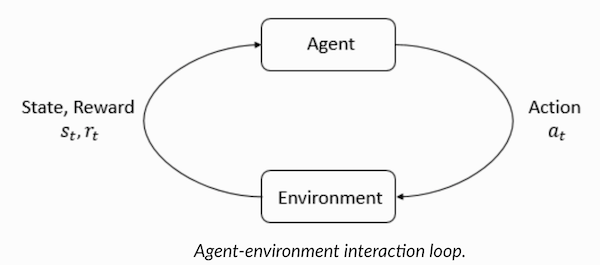
\includegraphics[width=1\linewidth]{RL_scheme}}
\caption{Схема метода обучения с подкреплением\cite{litlink19}.}
\label{ris:image}
\end{figure}\\
\textbf{Описание эксперимента}\\
В первую очередь, с помощью библиотеки OpenAI Gym была создана среда, в которой обучающийся агент производит какие-либо действия. В случае, рассматриваемом в данной работе, создается среда TetrisA-v0 — эмулятор игры "Тетрис". В этой среде агент может сделать ход, передав один из вариантов действий: сдвиг фигурки влево, сдвиг фигурки вправо, поворот на 90° по часовой стрелке, против часовой стрелки, ускорение падения фигурки. При заполнении строки частями фигурок среда автоматически очищает строку и добавляет 1 к награде.\\
\begin{figure}[h]
\center{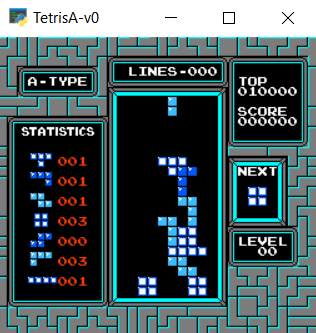
\includegraphics[width=\linewidth/3]{tetris_example}}
\caption{Пример среды TetrisA-v0.}
\label{ris:image}
\end{figure}\\
Затем с помощью библиотеки KerasRL была создана модель нейронной сети со следующими слоями. 1 слой, необходимый для сглаживания входных данных. Входными данными является информация, занята или свободна каждая клетка игрового поля. 2 сильно связанный слой с 24 входными синапсами и функцией активации выпрямленного линейного блока. Последний сильно связанный слой имеет линейную функцию активации и 12 выходных синапсов: каждый синапс отвечает за одно из действий.\\
\begin{figure}[h]
\center{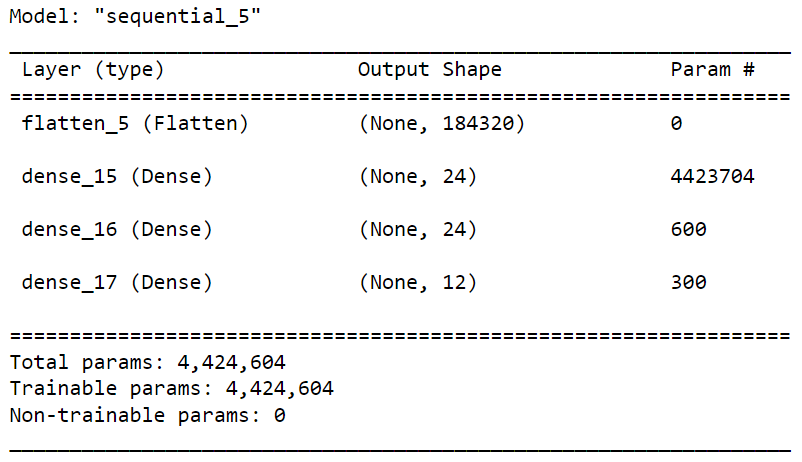
\includegraphics[width=\linewidth/2]{network}}
\caption{Краткое описание нейронной сети.}
\label{ris:image}
\end{figure}\\
На основе данной сети был создан агент с политикой BoltzmannQPolicy. Это означает, что агент вычисляет вид распределения значений, возвращаемых средой, и выбирает случайное действие на основе этого распределения.\\
После 50000 шагов, занявших 8 часов 11 минут, агент научился играть в "Тетрис" со среднем значением награды 11.02. При этом среднее число шагов до проигрыша было равно 4260.23.\\
\newpage
\begin{center}
\item\subsection{Применение обучения с подкреплением в основной задаче}
\end{center}
\textbf{Обзор и анализ источников}\\
Для сравнения результатов выбранного метода был выбран эвристический алгоритм, реализованный в фреймворке Protean. Его принцип работы описан в статье Protean: VM Allocation Service at Scale\cite{litlink21}. Приведенный в статье фреймворк используется в облачной платформе Microsoft Azure. Выбранный фреймворк покрывает все задачи распределения облачных ресурсов, но в данной статье будет использована только его часть для соотнесения результатов. Также для обучения агента будет использованы данные, приведенные в статье\cite{litlink22}.\\
В статье A Joint Resource Allocation, Security with Efficient Task Scheduling in Cloud Computing Using Hybrid Machine Learning Techniques\cite{litlink23} описан общий подход к применению машинного обучения в исследуемой задаче. Однако, обучение с подкреплением не было использовано в данной статье, что затрудняет сравнение результатов.\\
A Hierarchical Framework of Cloud Resource Allocation and Power Management Using Deep Reinforcement Learning\cite{litlink24} является одной из первых работ по применению RL в задаче распределения ресурсов в облаке. В ней описаны несколько алгоритмов, основанных на обучении с подкреплением, и каждый из них превосходит эвристический метод по различным метрикам.\\~\\
\textbf{Обзор исходных данных}\\
Рассмотим данные, на которых происходило обучение. Это Microsoft Azure Traces за две недели работы сервиса. Они состоят из двух частей — VM Requests и VM Types. Это запросы клиентов на выделение виртуальной машины нужных характеристик и база данных доступных серверов. 
\begin{figure}[h]
\center{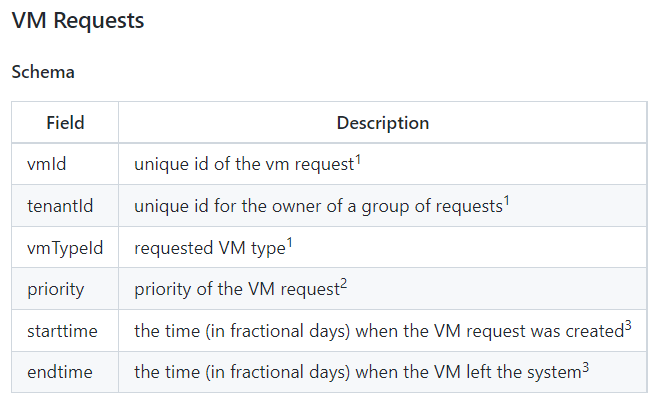
\includegraphics[width=\linewidth/2]{VMRequests}}
\caption{Схема базы данных запросов пользователей Microsoft Azure\cite{litlink22}.}
\label{ris:image}
\end{figure}
\begin{figure}[h]
\center{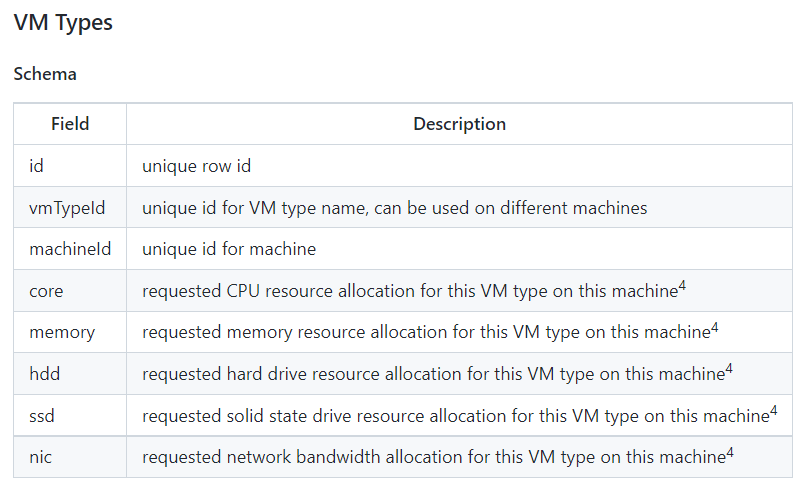
\includegraphics[width=\linewidth/2]{VMTypes}}
\caption{Схема базы данных доступных серверов Microsoft Azure\cite{litlink22}.}
\label{ris:image}
\end{figure}\\
\textbf{Реализация эвристического алгоритма}\\
В первую очередь, был повторен эвристический алгоритм, использованный в фреймворке Protean. Его псевдокод приведен в упомянутой выше статье. Выделение виртуальной машины клиенту происходит в нем в виде транзакции, чтобы обеспечить атомарность процесса. Каждый запрос добавляется в очередь на выделение виртуальной машины. Если же количество попыток выделить VM для данного запроса превышает установленное значение, он считается не обработанным.\\
\begin{figure}[h]
\center{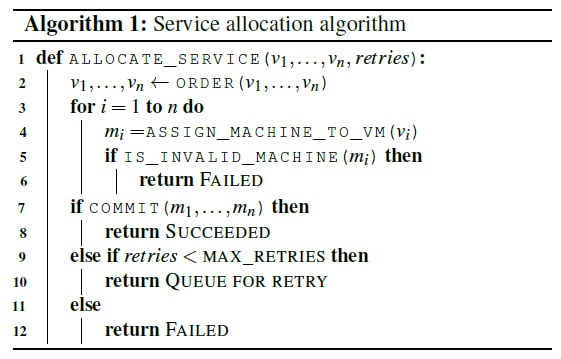
\includegraphics[width=\linewidth/2]{Algorithm}}
\caption{Описание эвристического алгоритма Protean\cite{litlink21}.}
\label{ris:image}
\end{figure}\\
Для удобства разработки, описанный алгоритм повторен в методологии ООП. Были созданы следующие классы: 
\begin{itemize}
\item VirtualMachine для хранения информации о виртуальной машине
\item Request для информации о каждом запросе клиента
\item Distributor, отвечающий за распределение приходящих запросов
\end{itemize}
Для реализации симуляции приходящих в реальном времени запросов была создана очередь событий. Использовался класс SortedList библиотеки sortedcontainers языка python. 
\begin{figure}[h!]
\center{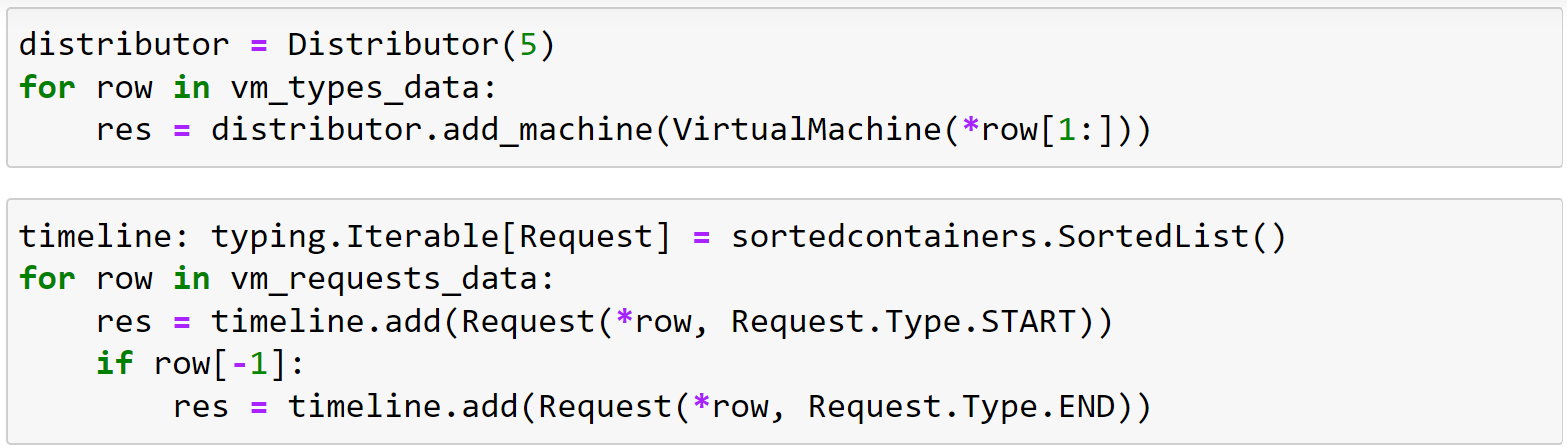
\includegraphics[width=\linewidth/2]{timeline}}
\caption{Симуляция запросов в реальном времени.}
\label{ris:image}
\end{figure}\\
Объект класса Distributor хранит метрики, которые характеризуют успешность распределения ресурсов:
\begin{itemize}
\item задержка
\item пропускная способность
\item число принятых запросов 
\end{itemize}
Данные метрики были взяты из статьи Protean: VM Allocation Service at Scale\cite{litlink21}. Задержка отражает время, которое запрос ожидал выделения сервера под его выполнение. Пропускная способность показывает, какое количество запросов было обработано в единицу времени. Число принятых запросов характеризует, сколько запросов удалось принять. Запрос может быть не принят из-за отсутствия подходящего сервера.\\
~\\
\begin{center}
\textbf{Результаты эвристического алгоритма}\\
\begin{tabular}{ | l | l | l | }
\hline
Метрика & Значение & Идеальное значение\\ \hline
Средняя задержка & 55 минут 14 секунд & 0 секунд \\
Пропускная способность & 13 333 запроса в час & Не ограничено \\
Общее число принятых запросов & 4 479 888 запросов & 5 559 800 запросов \\
\hline
\end{tabular}
\end{center}
~\\
\textbf{Описание эксперимента}\\
Для исследования области применимости RL в данной задаче были использованы те же классы Request и VirtualMachine. Но для распределения запросов создан новый класс RLDistibutor. В нем с помощью библиотеки KerasRL была создана модель нейронной сети. Ее архитектура взята из статьи A Hierarchical Framework of Cloud Resource Allocation and Power Management Using Deep Reinforcement Learning\cite{litlink24}. На первый слой подаются данные о занятости каждого из доступных серверов. Второй сильно связанный слой имеет линейную функцию активации и 50 выходных синапсов. Третий слой имеет функцию активации выпрямленного линейного блока и имеет 100 входных синапсов. Четвертый слой обладает аналогичной функцией активации и 50 синапсами. Последний слой реализует линейную функцию активации и имеет 4619 выходных синапсов — активация первого из которых определяет сервер, выделенный для текущего запроса. На основе описанной сети создан агент с политикой BoltzmannQPolicy.\\
\begin{figure}[h!]
\center{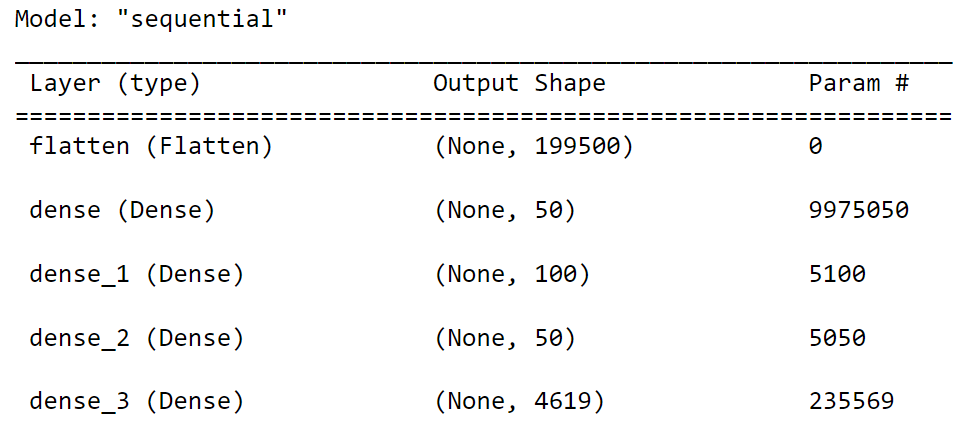
\includegraphics[width=\linewidth/2]{model_format}}
\caption{Архитектура нейронной сети.}
\label{ris:image}
\end{figure}\\
\textbf{Результаты эксперимента}\\
\begin{tabular}{ | l | l | l | l | }
\hline
Метрика & Эксперимент 1 & Эксперимент 2 & Идеальное значение\\ \hline
Средняя задержка & \textbf{92 минуты 15 секунд} & 97 минут 43 секунды & 0 секунд \\
Пропускная способность & 3 051 запрос в час & \textbf{4 666 запроса в час} & Не ограничено \\
Общее число принятых запросов & 1 025 136 запросов & \textbf{1 567 776 запросов} & 5 559 800 запросов \\
\hline
\end{tabular}
\begin{center}
\section {Заключение}
\end{center}
В данной научно-исследовательской работе изучен один из способов машинного обучения — обучение с подкреплением. В первой ее части рассмотрено применение обучения с подкреплением в задаче автоматической игры в "Тетрис". Проанализированы научные работы других авторов на эту тему, создана нейронная сеть и агент на ее основе. Полученный результат сравним со значениями, полученными авторами других статей.\\
Во второй части работы произведена попытка применения обучения с подкреплением в задаче распределения облачных ресурсов. Однако полученные результаты не являются удовлетворительными, так как в разы хуже альтернативного эвристического алгоритма.\\
~\\
Таким образом, исследовательская работа показывает, что обучение с подкреплением относительно успешно решает задачу автоматической игры в "Тетрис". Но вторая часть работы требует доработки. Выбранный в данной НИР вид нейронной сети решает поставленную задачу значительно хуже, чем эвристический алгоритм.\\
~\\
Первая часть работы выполнена полностью: показано успешное применение обучения с подкреплением. Работа может быть улучшена, если рассмотреть другие виды машинного обучения или другие архитектуры нейронной сети. Вторая часть работы требует дополнительного изучения. Необходимо рассмотреть большее количество вариантов архитектуры нейронной сети, чтобы убедиться в неработоспособности выбранного метода решения поставленной задачи или найти лучшее решение.\\
~\\
Код, полученный в ходе первой части работы может быть использован для решения задачи игры в "Тетрис" или в другую компьютерную игру, так как в нем использованы популярные библиотеки. Результаты второй части научно-исследовательской работы также могут быть применены на практике: разработан фреймворк, позволяющий в режиме реального времени распределять приходящие запросы на выделение облачных ресурсов. Однако подобное внедрение не является экономически оправданным, так как эвристический алгоритм показывает лучшие результаты.\\
~\\
Сравним полученный результат игры в "Тетрис" с другими реализациями RL применимо к данной задаче. В статье Playing the Original Game Boy Tetris Using a Real Coded Genetic Algorithm\cite{litlink7} средний результат алгоритма "FS-B" составил 30.71 ± 15.82, что является сравнимым с полученным значением. В работе Learn to Play Tetris with Deep Reinforcement Learning\cite{litlink20} алгоритмы Dreamer, Plan2xplore и LucidDreamer получили 55, 72 и 107 значений стертых линий, что является большим, но близким к полученному результатом. Таким образом, эксперимент с автоматической игрой в "Тетрис" показал, что RL является применимым к данной задаче алгоритмом и получает значимый результат.\\
~\\
Результат основной части работы значительно ниже эвристического алгоритма, описанного в статье Protean: VM Allocation Service at Scale\cite{litlink21}. При дальнейшем изучении данной темы возможно сравнение с алгоритмами, описанными в других статьях, например, A Joint Resource Allocation, Security with Efficient Task Scheduling in Cloud Computing Using Hybrid Machine Learning Techniques\cite{litlink23} или A Hierarchical Framework of Cloud Resource Allocation and Power Management Using Deep Reinforcement Learning\cite{litlink24}. Однако в данный момент сравнение с ними не представляется возможным, так как обучение происходило на разных входных данных.
\newpage
\begin{center}
\begin{thebibliography}{}
\bibitem{litlink1}  \textit{Kent, Steven} (2001) The Ultimate History of Video Games: From Pong to Pokemon: The Story Behind the Craze That Touched Our Lives and Changed the World (1st ed.). Three Rivers Press. С. 377-381. 
    \bibitem{litlink2}  \textit{Arif Mohamed} (2018) A history of cloud computing // Сайт Сomputerweekly.com. 9 апреля (https://www.computerweekly.com/feature/A-history-of-cloud-computing) Просмотрено: 11.12.2021.
    \bibitem{litlink3}  \textit{Matt Kapko} (2021) Can Huawei ‘Reinvent Itself’ as a Cloud Leader? // Сайт Sdxcentral.com. 26 апреля (https://www.sdxcentral.com/articles/news/can-huawei-reinvent-itself-as-a-cloud-leader/2021/04/) Просмотрено: 11.12.2021
    \bibitem{litlink4} \textit{Laura Wood} (2021) Global Cloud Computing Market (2020 to 2026) - by Service, Deployment, Application Type, End-user and Region Businesswire.com. 24 августа (https://www.businesswire.com/news/home/20210824005585/en/Global-Cloud-Computing-Market-2020-to-2026---by-Service-Deployment-Application-Type-End-user-and-Region---ResearchAndMarkets.com) Просмотрено: 11.12.2021
\bibitem{litlink5}  \textit{Erik D. Demaine, Susan Hohenberger, David Liben-Nowell} (2002) Tetris is Hard, Even to Approximate // Сайт Arxiv.org. 21 октября (https://arxiv.org/abs/cs/0210020) Просмотрено: 11.12.2021
\bibitem{litlink6}  \textit{Harvinder Singh, Anshu Bhasin, Parag Ravikant Kaveri} (2021) QRAS: efficient resource allocation for task scheduling in cloud computing // Сайт Researchgate.net. Апрель (https://www.researchgate.net/publication/350192028\_QRAS\_efficient\_resource\_allocation\_for\_task\_\\scheduling\_in\_cloud\_computing) Просмотрено: 11.12.2021
\bibitem{litlink7} \textit{Renan Samuel da Silva, Rafael Stubs Parpinelli} (2017) Playing the Original Game Boy Tetris Using a Real Coded Genetic Algorithm // Сайт Researchgate.net. Октрябрь (https://www.researchgate.net/publication/322321608\_Playing\_the\_Original\_Game\_Boy\_Tetris\_Using\_a\_\\Real\_Coded\_Genetic\_Algorithm) Просмотрено: 11.12.2021
\bibitem{litlink8} \textit{X. Chen, H. Wang, W. Wang, Y. Shi, and Y. Gao} (2009) Apply ant colony optimization to tetris // Сайт Dl.acm.org. 8 июля (https://dl.acm.org/doi/10.1145/1569901.1570136) Просмотрено: 11.12.2021
\bibitem{litlink9} \textit{L. Langenhoven, W. S. van Heerden, and A. P. Engelbrecht} (2010) Swarm tetris: Applying particle swarm optimization to tetris // Сайт Ieeexplore.ieee.org. 18-23 июля (https://ieeexplore.ieee.org/document/5586033) Просмотрено: 11.12.2021
\bibitem{litlink10} \textit{nuno-faria, nlinker (Nick Linker)} (2019) A bot that plays tetris using deep reinforcement learning. // Сайт Github.com. 7 сентября (https://github.com/nuno-faria/tetris-ai) Просмотрено: 11.12.2021
\bibitem{litlink11} \textit{Baekalfen (Mads Ynddal)} (2021) Game Boy emulator written in Python. // Сайт Github.com. 22 октября (https://github.com/Baekalfen/PyBoy) Просмотрено: 01.02.2022
\bibitem{litlink12} \textit{Christian Kauten} (2019) An OpenAI Gym environment for Tetris on The Nintendo Entertainment System (NES) based on the nes-py emulator. // Сайт Pypi.org. 3 июня (https://github.com/Baekalfen/PyBoy) Просмотрено: 01.02.2022
\bibitem{litlink13} \textit{OpenAI} (2021) A toolkit for developing and comparing reinforcement learning algorithms. // Сайт Github.com. 2 октября (https://github.com/openai/gym) Просмотрено: 01.02.2022
\bibitem{litlink14} \textit{accel-brain, chimera0} (2020) Reinforcement Learning Library: pyqlearning. // Сайт Pypi.org. 13 июля (https://pypi.org/project/pyqlearning/) Просмотрено: 01.02.2022
\bibitem{litlink15} \textit{Tensorforce} (2021) Tensorforce: a TensorFlow library for applied reinforcement learning. // Сайт Github.com. 30 августа (https://github.com/tensorforce/tensorforce) Просмотрено: 01.02.2022
\bibitem{litlink16} \textit{Keras-RL} (2018) Deep Reinforcement Learning for Keras. // Сайт Github.com. 1 мая (https://github.com/keras-rl/keras-rl) Просмотрено: 01.02.2022
\bibitem{litlink17} \textit{tensorflow} (2021) An Open Source Machine Learning Framework for Everyone. // Сайт Github.com. 4 ноября (https://github.com/tensorflow/tensorflow) Просмотрено: 01.02.2022
\bibitem{litlink18} \textit{Cade Metz} (2015) TensorFlow, Google's Open Source AI, Signals Big Changes in Hardware Too. // Сайт Wired.com. 10 ноября (https://www.wired.com/2015/11/googles-open-source-ai-tensorflow-signals-fast-changing-hardware-world/) Просмотрено: 02.02.2022
\bibitem{litlink19} \textit{Vihar Kurama, Samhita Alla} (2018) Обучение с подкреплением на языке Python. // Сайт Habr.com. 28 декабря (https://habr.com/ru/company/piter/blog/434738/) Просмотрено: 02.02.2022
\bibitem{litlink20} \textit{Hanyuan Liu, Lixin Liu} (2020) Learn to Play Tetris with Deep Reinforcement Learning. // Сайт Openreview.net. 14 декабря (https://openreview.net/forum?id=8TLyqLGQ7Tg) Просмотрено: 05.05.2022
\bibitem{litlink21} \textit{Ori Hadary, Luke Marshall, Ishai Menache, Abhisek Pan, Esaias E Greeff, David Dion, Star Dorminey, Shailesh Joshi, Yang Chen, Mark Russinovich, and Thomas Moscibroda} (2020) Protean: VM Allocation Service at Scale. // Сайт Usenix.org. 4-6 ноября (https://www.usenix.org/conference/osdi20/presentation/hadary) Просмотрено: 05.05.2022
\bibitem{litlink22} \textit{elicortez, rfonseca, SamehElnikety} (2020) AzurePublicDataset. // Сайт Github.com. 13 ноября (https://github.com/Azure/AzurePublicDataset/blob/master/AzureTracesForPacking2020.md) Просмотрено: 05.05.2022
\bibitem{litlink23} \textit{Prasanta Kumar Bal, Sudhir Kumar Mohapatra, Tapan Kumar Das, Kathiravan Srinivasan and Yuh-Chung Hu} (2022) A Joint Resource Allocation, Security with Efficient Task Scheduling in Cloud Computing Using Hybrid Machine Learning Techniques. // Сайт Researchgate.net. 13 ноября (https://www.researchgate.net/publication/358396471\_A\_Joint\_Resource\_Allocation\_Security\_with\_Efficient\\\_Task\_Scheduling\_in\_Cloud\_Computing\_Using\_Hybrid\_Machine\_Learning\_Techniques) Просмотрено: 05.05.2022
\bibitem{litlink24} \textit{Ning Liu, Zhe Li, Zhiyuan Xu, Jielong Xu, Sheng Lin, Qinru Qiu, Jian Tang, Yanzhi Wang} (2017) A Hierarchical Framework of Cloud Resource Allocation and Power Management Using Deep Reinforcement Learning. // Сайт Arxiv.org. 13 марта (https://arxiv.org/abs/1703.04221) Просмотрено: 05.05.2022
\end{thebibliography}
\end{center}
\newpage
\begin{center}
\section {Приложения}
\end{center}
\zz{}\textbf{Приложение 1\\}
Ссылка на репозиторий проекта с исходным кодом и всеми использованными материалами.\\
https://github.com/NikPeg/Reinforcement-learning-for-resource-allocation-tasks-in-the-cloud
\end{document}